% Diagram: Inference Lifecycle
\begin{figure}[htbp]
\centering
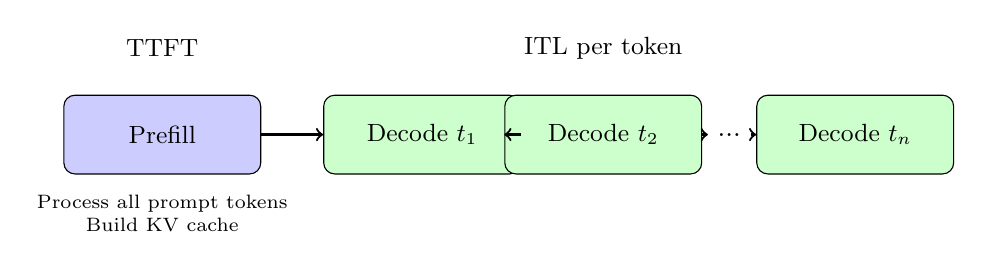
\begin{tikzpicture}[
    node distance=0.8cm,
    phase/.style={rectangle, draw, rounded corners, minimum width=2.5cm, minimum height=1cm, font=\small},
    prefill/.style={phase, fill=blue!20},
    decode/.style={phase, fill=green!20},
    arrow/.style={->, thick}
]
% Prefill
\node[prefill] (pf) {Prefill};
\node[below of=pf, yshift=-0.2cm, font=\scriptsize, align=center] (pf-desc) {Process all prompt tokens\\Build KV cache};

% Decode steps
\node[decode, right of=pf, xshift=2.5cm] (d1) {Decode $t_1$};
\node[decode, right of=d1, xshift=1.5cm] (d2) {Decode $t_2$};
\node[right of=d2, xshift=0.8cm] (dots) {...};
\node[decode, right of=dots, xshift=0.8cm] (dn) {Decode $t_n$};

% Arrows
\draw[arrow] (pf) -- (d1);
\draw[arrow] (d1) -- (d2);
\draw[arrow] (d2) -- (dots);
\draw[arrow] (dots) -- (dn);

% Labels
\node[above of=pf, yshift=0.3cm, font=\small] {TTFT};
\node[above of=d2, yshift=0.3cm, font=\small] {ITL per token};

\end{tikzpicture}
\caption{Inference lifecycle: prefill determines TTFT, decode determines generation speed.}
\label{fig:inference-lifecycle}
\end{figure}
